\section{Durchführung}
\label{sec:Durchführung}

In \autoref{fig:Abb_3} ist der gegebene Lock-In-Verstärker dargestellt.
\begin{figure}[H]
    \centering
    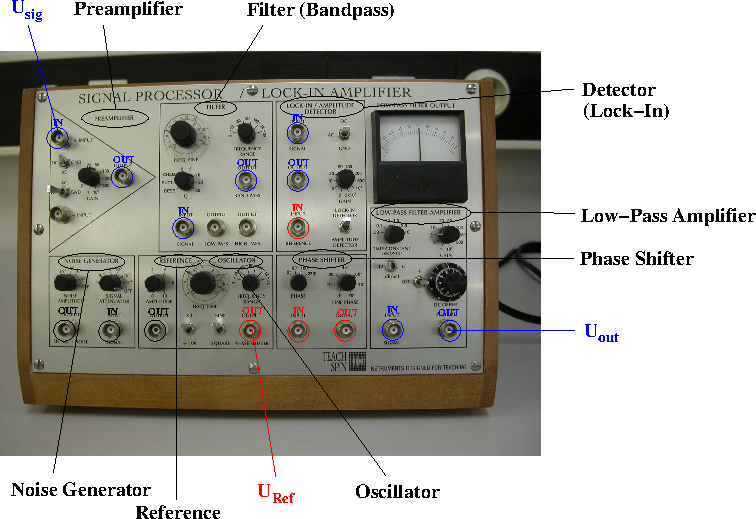
\includegraphics[width=0.7\textwidth]{build/Abb_3.pdf}
    \caption {Der Lock-In-Verstärker.\cite{V303}}
    \label{fig:Abb_3}
\end{figure}
Zunächst wird am Funktionsgenerator (Referece/Oscillator) geprüft, an welchem Ausgang die Spannung veränderlich ist und an welchem eine konstante Amplitude generiert wird.
Um die Abhängigkeit von der Spannung zu der Phase zu zeigen wird die Schaltung gemäß \autoref{fig:Abb_4} aufgebaut, wobei der Noise Generator zunächst überbrückt wird.
\begin{figure}[H]
    \centering
    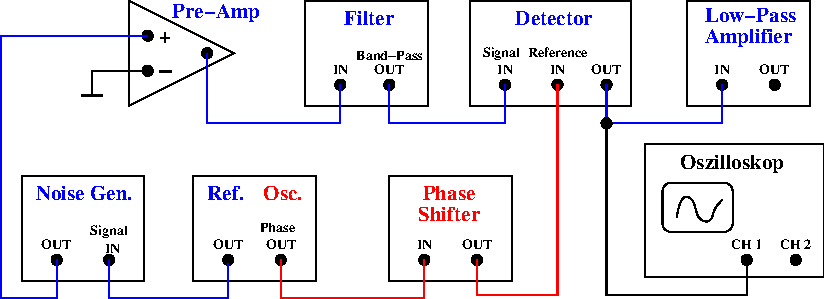
\includegraphics[width=0.7\textwidth]{build/Abb_4.pdf}
    \caption {Schematischer Aufbau eines Lock-In-Generators.\cite{V303}}
    \label{fig:Abb_4}
\end{figure}
Es wird ein Sinussignal mit dem Funktionsgenerator erzeugt.
Die Amplitude der Ausgangspannung wird für neun verschiedene Phasen im Abstand $\qty{45}{\degree}$ am Oszilloskop gemessen und auf einem USB-Stick gespeichert.
Dies wird mit zugeschaltetem Noise Generator wiederholt.\\
\\
Nun wird die Schaltung wie in \autoref{fig:Abb_5} aufgebaut.
\begin{figure}[H]
    \centering
    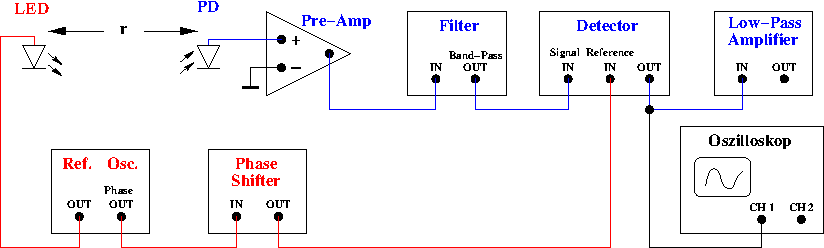
\includegraphics[width=0.7\textwidth]{build/Abb_5.pdf}
    \caption {Photodetektorschaltung.\cite{V303}}
    \label{fig:Abb_5}
\end{figure}
Es wird die von der Photodiode empfangene Lichtintensität der LED in Abhängigkeit vom Abstand zwischen LED und Photodiode untersucht.
Dafür wird die LED in $\qty{5}{\centi\meter}$ Abständen weiter weg von der Photodiode geschoben und die jeweilige Spanunngsamplitude notiert.

